\chapter{Аналитическая часть}

В данном разделе представлено описание объектов сцены, а также обоснован выбор алгоритмов, которые будут использованы для ее визуализации.

\section{Формализация объектов сцены}

Сцена состоит из следующих объектов:

\begin{itemize}[label=---]
	\item точечного источника света --- задается положением в пространстве и интенсивностью;
	\item источника дыма --- задается положением в пространстве;
	\item модели дыма;
	\item комнаты --- пространство в пределах, которого будет распространяться дым;
\item предметов интерьера --- объекты внутри комнаты, мешающие распространению дыма и света.
\end{itemize}

\section{Обоснование выбора формы задания трехмерных моделей}

Отображением формы и размеров объектов являются модели. Обычно используются три формы задания моделей.

\begin{enumerate}
	\item Каркасная (проволочная) модель.
	Одна из простейших форм задания модели, так как мы храним информацию только о вершинах и ребрах нашего объекта.
	\item Поверхностная модель.
	Поверхностная модель объекта — это оболочка объекта, пустая внутри. Такая информационная модель содержит данные только о внешних геометрических параметрах объекта. При этом могут использоваться различные типы поверхностей, ограничивающих объект, такие как полигональные модели, поверхности второго порядка и др.
	\item Объемная (твердотельная) модель.
	При твердотельном моделировании учитывается еще материал, из которого изготовлен объект, т.е. у нас есть информация о том, с какой стороны поверхности расположен материал.
	Для решения данной задачи лучше всего подойдет поверхностная модель. Каркасные модели могут привести к неправильному восприятию формы объекта, а реализация объемной модели избыточна и потребует дополнительного количества ресурсов.
\end{enumerate}

\subsection{Способы задания поверхностных моделей}

На следующем шаге необходимо определиться со способом задания поверхностной модели.
\begin{enumerate}
	\item Аналитический способ.
	Этот способ задания модели характеризуется описанием модели объекта, которое доступно в неявной форме, то есть для получения визуальных характеристик необходимо дополнительно вычислять некоторую функцию, которая зависит от параметра.
	\item Полигональная сетка.
	Данный способ характеризуется совокупностью вершин, граней и ребер, которые определяют форму многогранного объекта в трехмерной компьютерной графике.
\end{enumerate}

\subsection{Способы хранения поверхностных моделей}
Существует несколько способов хранения информации о сетке.
\begin{enumerate}
	\item Список граней.
	Объект – это множество граней и множество вершин. В каждую грань входят как минимум 3 вершины.
	\item «Крылатое» представление.
	Каждая точка ребра указывает на две вершины, две грани и четыре ребра, которые её касаются.
	\item Полурёберные сетки.
	То же «крылатое» представление, но информация обхода хранится для половины грани.
	\item Таблица углов.
	Это таблица, хранящая вершины. Обход заданной таблицы неявно задаёт полигоны. Такое представление более компактно и более производительно для нахождения полигонов, но, в связи с тем, что вершины присутствуют в описании нескольких углов, операции по их изменению медленны.
	\item Вершинное представление.
	Хранятся лишь вершины, которые указывают на другие вершины. Простота представления даёт возможность проводить над сеткой множество операций.
\end{enumerate}

\subsection*{Вывод}

Одним из важнейших факторов в выборе способа реализации модели является скорость вычисления преобразований над объектом. Поэтому для задания модели наилучшим представлением будет полигональная сетка. При этом способ хранения полигональной сетки --- список граней. Такое представление является наиболее простым. Также этот метод дает возможность быстрого преобразования модели, потому что структура будет включать в себя список вершин. 

\section {Обоснование выбора формы задания дыма}

Дым представляет собой дисперсную систему, состоящую из твердых частиц, находящихся во взвешенном состоянии.

\subsection{Уравнения Навье-Стокса}

Поведение частиц дыма аналогично поведению легких газов. Частицы дыма легкие и мелкие, и при испускании из неподвижного источника, такого как свеча, не будут иметь скорости. Движение частиц в основном вызывают окружающие силы. Частицы дыма не влияют на свое собственное движение, а зависят исключительно от внешних сил, толкающих и тянущих их в разных направлениях. Дым, как правило, вытягивается вверх из-за малого веса частиц, которые следуют за теплым воздушным потоком, поднимающимся вверх. Дым, как и жидкости, также будет растекаться по поверхностям при взаимодействии с объектами. Для моделирования такого поведения часто используется вычислительная гидродинамика. Обычно используемыми уравнениями для решения CFD являются уравнения Навье-Стокса и Эйлера. Оба уравнения описывают, как изменяются скорости и массы. При условии, что вязкость равна нулю, удаление теплопроводности из уравнения Навье-Стокса дает уравнение Эйлера \cite{cfd}. 
\begin{equation}
	\frac{\partial \vec{u}}{\partial x} = -(\vec{u}\cdot\nabla) \vec{u} - \frac{1}{\rho} \nabla p + \vec{f} \text{,}
\end{equation}
где
$\rho$ --- плотность,

$p$ --- давление,

$\vec{f}$ --- произвольная сила,

$\vec{u}$ --- скорость частицы.
\subsection{Система частиц}

\textbf{Движение частиц} \cite{smokeparticle}.

Основное движение дыма происходит вверх по спирали. Очевидно, что для достижения более хаотичного движения, потребуется добавление 3D-шума. Спираль, по которой движутся частицы, управляется простым векторным полем \ref{particle_move}.

\begin{equation}
	\label{particle_move}
	F(xpos,ypos,zpos) = \{ 2 \cdot zpos\cdot ypos,yvel,-2\cdot xpos\cdot ypos \} \text{,}
\end{equation}
где $xpos$, $ypos$ и $zpos$ - мировые координаты частицы, а $yvel$ - скорость, с которой частицы движутся вверх.

Это значение одинаково везде в пространстве. Сила тяжести не оказывает значительное влияние на частицы дыма и не принимается во внимание. Также не происходит столкновений между частицами дыма.

Частицам присваиваются скорости в соответствии с их положением в векторном поле. Затем вычисляются их новые позиции.
\begin{equation}
p(t + dt) = p(t) + \vec{v}\cdot dt\text{,}
\end{equation}

где $p(t)$ - положение частицы в момент времени t, а $\vec{v}$ - трехмерный вектор, представляющий скорость частицы, заданную векторным полем.
 
Конечно, это не конечное положение частицы. Шум добавляется для создания более хаотичного движения. Все частицы рождаются со скоростью (0,1,0). Частицы перемещаются в соответствии с их текущей скоростью, прежде чем им присваивается новая скорость.

\textbf{Шум частиц}.

Шум, используемый для частиц, отличается от обычного шума главным образом возвращаемым из него значением. Обычный шум возвращает значение от нуля до единицы, тогда как шум, используемый для системы частиц, возвращает 3D-вектор.
 
\textbf{Время жизни частицы}.

Все частицы абсолютно идентичны при рождении. В промежутках между кадрами сохраняются положение, скорость и возраст частиц. В начале каждого кадра рождается фиксированное количество частиц. Частицы удаляются, когда они превысили максимальный возраст частиц, который является глобальным и, следовательно, одинаковым для всех частиц.

\subsection*{Вывод}
Хотя CFD метод даст более реалистичное изображение, он очень сложен в реализации и требует большой вычислительной мощности. Из-за таких серьезных недостатков для выполнения проекта был выбран метод, основанный на частицах.

\section{Выбор алгоритма удаления невидимых ребер и поверхностей}
 
Выбранный алгоритм удаления невидимых ребер должен обладать некоторым радом свойств, а именно:
\begin{itemize}[label=---]
	\item из-за большого количества частиц, алгоритм должен использовать минимум памяти;
	\item алгоритм должен быть достаточно быстрым;
	\item как результат работы алгоритм должен выдавать максимально реалистичное изображение.
\end{itemize}

\subsection{Алгоритм, использующий Z-буфер}

Суть данного алгоритма заключается в использовании двух буферов: буфера кадра, в котором хранятся атрибуты каждого пикселя, и Z-буфера, в котором хранится информация о координате Z для каждого пикселя. 

Первоначально в Z-буфере находятся минимально возможные значения Z, а в буфере кадра располагаются пиксели, описывающие фон. Каждый многоугольник преобразуется в растровую форму и записывается в буфер кадра. 

В процессе подсчета глубины нового пикселя, он сравнивается с тем значением, которое уже лежит в Z-буфере. Если новый пиксель расположен ближе к наблюдателю, чем предыдущий, то он заносится в буфер кадра и происходит корректировка Z-буфера.
 
Для решения задачи вычисления глубины Z каждый многоугольник описывается уравнением \ref{zbufer}.
\begin{equation}
	\label{zbufer}
	 ax+by+cz+d=0.
\end{equation}  
При $c=0$ многоугольник для наблюдателя вырождается в линию. 

Для некоторой сканирующей строки $y=const$, поэтому имеется возможность рекуррентно высчитывать $z^\prime$ \ref{zbuf2}.
\begin{equation}
	\label{zbuf2}
	\forall x^\prime=x+dx : z^\prime-z=-\frac{ax^\prime+d}{c}+\frac{ax+d}{c}=\frac{a(x-x^\prime)}{c}
\end{equation}

Получим $z^\prime=z-\frac{a}{c}$, так как $x-x^\prime=dx=1$.

При этом стоит отметить, что для невыпуклых многогранников предварительно потребуется удалить не лицевые грани.

\textbf{Преимущества}
\begin{itemize}[label=---]
	\item простота реализации; 
	\item оценка трудоемкости линейна. 
\end{itemize}

\textbf{Недостатки} 
\begin{itemize}[label=---]
	\item сложная реализация прозрачности; 
	\item большой объем требуемой памяти. 
\end{itemize}

\subsection{Алгоритм обратной трассировки лучей}
Из виртуального глаза через каждый пиксель изображения испускается луч и находится точка его пересечения с поверхностью сцены \cite{raytrace}.
Лучи, выпущенные из глаза называют первичными. 
Пусть, первичный луч пересекает некий объект 1 в точке H1.

Далее необходимо определить для каждого источника освещения, видна ли из него эта точка. 
Тогда к каждому точечному источнику света испускается теневой луч из точки H1.  
Если теневой луч находит пересечение с другими объектами, расположенными ближе чем источник света, значит, точка H1 находится в тени от этого источника. 
Иначе, освещение считается по некоторой локальной модели. 
\newpage
\textbf{Преимущества}
\begin{itemize}[label=---]
	\item высокая реалистичность синтезируемого изображения; 
	\item работа с поверхностями в математической форме; 
	\item вычислительная сложность слабо зависит от сложности сцены.
\end{itemize}

\textbf{Недостатки} --- скорость выполнения. 

\subsection{Алгоритм Робертса} 

Данный алгоритм работает в объектном пространстве, решая задачу только с выпуклыми телами. Алгоритм выполняется в 3 этапа. 

\textbf{Этап подготовки исходных данных.}

На данном этапе должна быть задана информация о телах. Для каждого тела сцены должна быть сформирована матрица тела $V$. Размерность матрицы --- $4n$, где $n$ --- количество граней тела. 

Каждый столбец матрицы представляет собой четыре коэффициента уравнения плоскости $ax+by+cz+d=0$, проходящей через очередную грань. 

Матрица тела должна быть сформирована корректно, то есть любая точка, расположенная внутри тела, должна располагаться по положительную сторону от каждой грани тела. В случае, если для очередной грани условие не выполняется, соответствующий столбец матрицы надо умножить на $-1$. 

\textbf{Этап удаления рёбер, экранируемых самим телом.}

На данном этапе рассматривается вектор взгляда $E = \{0, 0, -1, 0\}$. Для определения невидимых граней достаточно умножить вектор $E$ на матрицу тела $V$. Отрицательные компоненты полученного вектора будут соответствовать невидимым граням. 

\textbf{Этап удаления невидимых рёбер, экранируемых другими телами сцены.}

На данном этапе для определения невидимых точек ребра требуется построить луч, соединяющий точку наблюдения с точкой на ребре. Точка будет невидимой, если луч на своём пути встречает в качестве преграды рассматриваемое тело. 

\textbf{Преимущества}
\begin{itemize}[label=---]
	\item работа в объектном пространстве;
	\item высокая точность вычисления. 
\end{itemize}

\textbf{Недостатки}
\begin{itemize}[label=---]
	\item рост сложности алгоритма – квадрат числа объектов; 
	\item тела сцены должны быть выпуклыми (усложнение алгоритма, так как нужна будет проверка на выпуклость); 
	\item сложность реализации. 
\end{itemize}

\subsection{Алгоритм художника} 

Предназначен для изображения произвольных поверхностей. Принцип его работы заключается в выводе на экран объектов по мере их приближения к наблюдателю. Наиболее распространенная реализация алгоритма – сортировка по глубине, которая заключается в том, что произвольное множество граней сортируется по ближнему расстоянию от наблюдателя, а затем отсортированные грани выводятся на экран в порядке от самой дальней до самой ближней. 

Данный метод работает лучше для построения сцен, в которых отсутствуют пересекающиеся грани. 

\textbf{Преимущества} --- требование меньшей памяти, чем, например, алгоритм Z-буфера. 

\textbf{Недостатки}
\begin{itemize}[label=---]
	\item невысокая реалистичность изображения;
	\item сложность реализации при пересечения граней на сцене. 
\end{itemize}

\subsection{Алгоритм Варнока}

Алгоритм Варнока является одним из примеров алгоритма, основанного на разбиении картинной плоскости на части, для каждой из которых исходная задача может быть решена достаточно просто. Поскольку алгоритм Варнока нацелен на обработку картинки, он работает в пространстве изображения. 

В пространстве изображения рассматривается окно и решается вопрос о том, пусто ли оно, или его содержимое достаточно просто для визуализации. Если это не так, то окно разбивается на фрагменты до тех пор, пока содержимое фрагмента не станет достаточно простым для визуализации или его размер не достигнет требуемого предела разрешения. Сравнивая область с проекциями всех граней, можно выделить случаи, когда изображение, получающееся в рассматриваемой области, определяется сразу:

\begin{itemize}[label=---]
	\item проекция ни одной грани не попадает в область;
	\item проекция только одной грани содержится в области или пересекает область, то в этом случае проекции грани разбивают всю область на две части, одна из которых соответствует этой проекции;
	\item существует грань, проекция которой полностью накрывает данную область, и эта грань расположена к картинной плоскости ближе, чем все остальные грани, проекции которых пересекают данную область, то в данном случае область соответствует этой грани.
\end{itemize}

Если ни один из рассмотренных трех случаев не имеет места, то снова разбиваем область на четыре равные части и проверяем выполнение этих условий для каждой из частей. Те части, для которых таким образом не удалось установить видимость, разбиваем снова и т. д. 

\textbf{Преимущества} --- меньшие затраты по времени в случае области, содержащий мало информации. 

\textbf{Недостатки}
\begin{itemize}[label=---]
	\item алгоритм работает только в пространстве изображений;
	\item большие затраты по времени в случае области с высоким информационным содержимым. 
\end{itemize}

\subsection*{Вывод}
 
Для удаления невидимых линий выбран алгоритм обратной трассировки лучей. Этот алгоритм не только поможет добиться наибольшей реалистичности изображения, но и также позволит легко смоделировать распространение света в пространстве, согласно законам геометрической оптики. Данный алгоритм можно улучшить, если добавить в него обработку особых световых явлений. Помимо всего прочего данный алгоритм позволит построить качественные тени. Также немаловажен тот факт, что алгоритм трассировки лучей намного менее требователен к памяти, алгоритм Z-буфера.

\section{Анализ и выбор модели освещения}
Физические модели материалов стараются аппроксимировать свойства некоторого реального материала. Такие модели учитывают особенности поверхности материала или же поведение частиц материала. Эмпирические модели материалов устроены иначе, чем физически обоснованные. Данные модели подразумевают некий набор параметров, которые не имеют физической интерпретации, но которые позволяют с помощью подбора получить нужный вид модели. В данной работе следует делать выбор из эмпирических моделей, а конкретно из модели Ламберта и модели Фонга. 

\subsection{Модель Ламберта}
Модель Ламберта моделирует идеальное диффузное освещение, то есть свет при попадании на поверхность рассеивается равномерно во все стороны.
Интенсивность диффузного света приблизительно подчиняется закону Ламберта, то есть интенсивность пропорциональна только косинусу угла между направлением падающего света и нормалью к поверхности в точке отражения \ref{fig:lambert}. 

\begin{figure}[H]
	\centering
	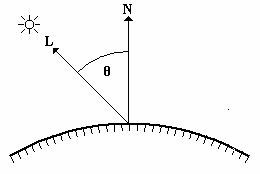
\includegraphics[width=1\linewidth]{inc/img/lambert}
	\caption[]{Модель освещения Ламберта}
	\label{fig:lambert}
\end{figure}

\begin{equation}
	I_d=I_0 \cdot \cos(\theta)
\end{equation}

\begin{equation}
	\cos(\theta)=\vec{L}\cdot\vec{N}
\end{equation}							

\begin{equation}
	I_d=I_0\cdot(\vec{L}\cdot\vec{N})
\end{equation}

Эта модель является одной из самых простых моделей освещения и очень часто используется в комбинации с другими моделями. Она может быть очень удобна для анализа свойств других моделей, за счет того, что ее легко выделить из любой модели и анализировать оставшиеся составляющие. 

\subsection{Модель Фонга}

Это классическая модель освещения. Модель представляет собой комбинацию диффузной и зеркальной составляющих. Работает модель таким образом, что кроме равномерного освещения на материале могут появляться блики. Местонахождение блика на объекте определяется из закона равенства углов падения и отражения. Чем ближе наблюдатель к углам отражения, тем выше яркость соответствующей точки. Падающий и отраженный лучи лежат в одной плоскости с нормалью к отражающей поверхности в точке падения \ref{fig:phong}.
\begin{figure}[H]
	\centering
	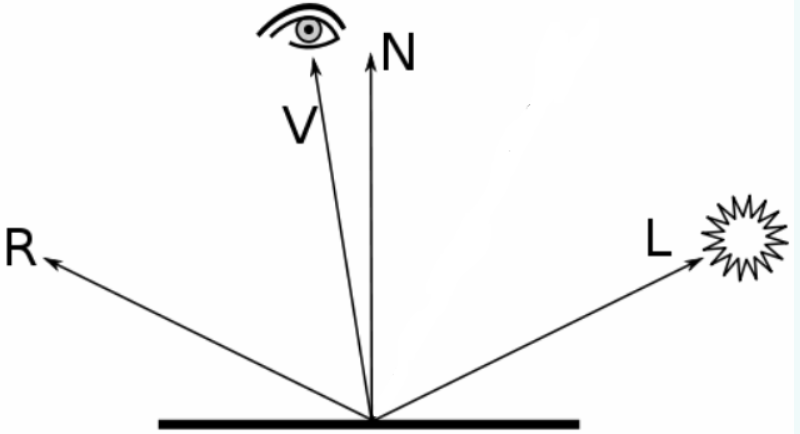
\includegraphics[width=1\linewidth]{inc/img/phong}
	\caption[]{Модель освещения Фонга}
	\label{fig:phong}
\end{figure}
\begin{equation}
	I={I_ak}_a+I_dk_d\cdot\left(\vec{N},\ \vec{L}\right)+I_sk_s\cdot{(\vec{V},\vec{R})}^p\text{,}
\end{equation}

где $k_a$ --- коэффициент фонового освещения,

$k_d$ --- коэффициент рассеянного освещения,

$k_s$ --- коэффициент бликового освещения,

$\vec{N}$ --- вектор нормали к поверхности,

$\vec{L}$ --- вектор направления падающего луча,
 
$\vec{R}$ --- вектор направления отраженного луча,

$\vec{V}$ --- вектор взгляда,

$p$ --- контрастность блика.

\subsection*{Вывод}
В качестве модели освещения в данной работе была выбрана модель Ламберта из-за своей простоты по сравнению с моделью Фонга. На расчет данных для модели Ламберта потребуется выполнить меньше вычислений, а значит ее реализация будет проще и потребует меньшего количества времени. 
\section*{Вывод} 
В данном разделе был проведен анализ алгоритмов удаления невидимых линий и модели освещения, которые возможно использовать для решения поставленных задач, а также выбраны формы задания дыма и объектов на сцене. В качестве ключевого алгоритма, выбран алгоритм обратной трассировки лучей, который будет реализован в рамках курсового проекта по компьютерной графике.

